\setstretch{1.0}
\chapter{Measuring Functional Connectivity in MEG}\label{chapter_fc_and_leakage}

In this chapter, the commonly used methods to measure functional connectivity using source reconstructed data are introduced. Whilst not intended as an exhaustive review of every connectivity metric, it covers many of the technical aspects that need to be addressed for a successful study. Also in this chapter the concept of signal leakage is introduced. This arises from source reconstruction errors and, if not carefully controlled for, will confound results. We introduce a model to characterise and correct for signal leakage, allowing for a confident assessment of functional connectivity. 

\doublespacing

\section*{Introduction}
Following the projection of MEG data into source space, achieved (in the case of this thesis) with beamforming, we can now turn our attention to the main focus of this thesis, the assessment of the functional connections within the brain. To reiterate Chapter \ref{chap_intro}, functional connections are defined as a \textit{statistical interdependency} between measured activity at two (or more) spatially separate regions of the brain \citep{Friston2011}. In fMRI, the term "functional connectivity" has become synonymous with the correlation of BOLD timecourses, but for MEG, the definition is considerably broader. The rich content of MEG data allows functional connectivity to be derived in many different ways, and whilst a number of types of coupling have become prominent, two in particular stand out for their popularity. The first arises from a fixed phase relationship between band-limited oscillatory signals (i.e. phase synchronisation), the second is the result of synchronisation between the amplitude envelopes of band limited oscillations; these will be discussed in more detail throughout the chapter.

Despite the advantages of source space estimation discussed in Chapter \ref{chapter_meg_source}, a significant technical confound arises from source reconstruction, which is typically termed “signal leakage”. The ill-posed nature of the MEG inverse problem \citep{Hadamard1902} causes a degree of spatial blurring in source space reconstruction. This means that a single point source will appear to spread across a finite volume. In addition to this spread, it is also possible for sources to be mislocalised, for example due to inaccuracies in modelling the forward vector or because of deviations from the assumptions driving the inverse model. This has a profound effect on functional connectivity calculations, as it has the tendency to artefactually inflate connectivity levels between regions. 

In this chapter we discuss the techniques to measure functional connectivity without the confound of signal leakage.  Section \ref{sec_fc_1} gives a brief overview of popular methods to assess functional connectivity. Section \ref{sec_signal_leakage} introduces the problems of artefactual functional connectivity as the result of signal leakage, with the aid of an analytical model and simulations, with Section \ref{sec_signal_corr} discussing potential solutions.

\section{Functional Connectivity Methods}\label{sec_fc_1}

At its simplest, functional connectivity measures the relation between two time series; but so rich are the properties of the MEG signal, that many different tests could be considered. In a review on functional connectivity by \cite{Engel2013}, they suggest that there are two types of intrinsic coupling modes (ICMs)\footnote{Admittedly, this does over simplify the wider picture, as there are methods which look at phase-amplitude coupling \citep{Canolty2006,Florin2015} and those which asses coupling across frequencies \citep{Canolty2010,vanWijk2014}, but the two catagories mentioned in the main text are by far the most popular.}, those which assess the relation of power between two signals (Envelope coupling), and those which look at the synchrony of the data based on their phase (Phase coupling). Examples of this are illustrated in Figure \ref{figure_3_a}. 

\begin{figure}[h!]
	\begin{center}
		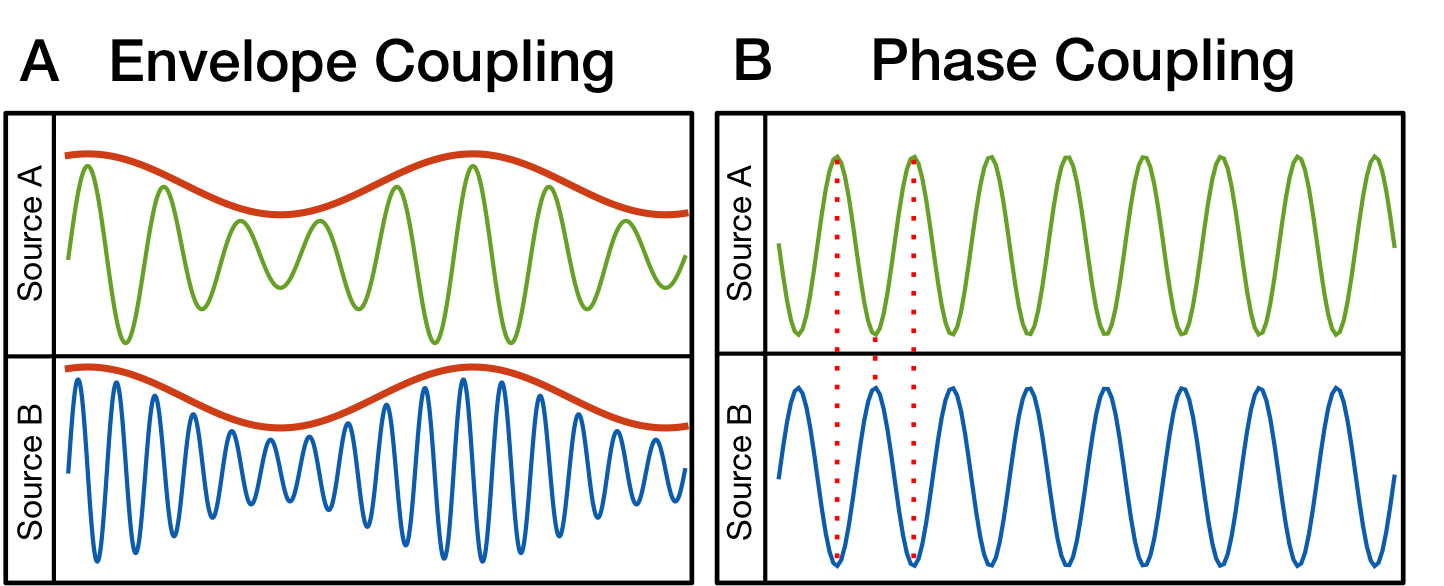
\includegraphics[width=0.9\linewidth]{./images/chapter3/fig_conn_1.png}\caption{Schematic diagram of phase and envelope based connectivity analyses based upon neural oscillations. A) Envelope coupling is based upon correlation between the oscillatory envelopes of two band limited sources. B) Phase coupling typically seeks to quantify the relation of the phases of two signals, in this case the two signals have a constant difference of π.}\label{figure_3_a}
	\end{center}
\end{figure}

These two categories of coupling methods, which focus on different aspects of the MEG signal, tend to reveal different parts of the wider functional connectivity picture \citep{Scholvinck2013}. Amplitude connectivity tends to better resemble the long range connections seen in fMRI and phase based measurements less so \citep{Brookes2011a,Tewarie2016}. This is possibly reflected in invasive measurements where amplitude correlations appear to be longer ranging than correlation of the raw signals \citep{Leopold2003}. However that is not to say that phase based measurements do not have their place in electrophysiological functional connectivity analysis, as they have been used successfully in many electrophysiological studies \citep{Gross2001,Nolte2004,Jerbi2007,Kujala2007,Guggisberg2008,Hillebrand2012,Marzetti2013}. Support for a multi-metric analysis (one which combines amplitude and phase connectivity assessments) has been shown in a recent study, where combination of concurrent phase and amplitude connectivity measurements better predict the connectivity patterns seen in fMRI than either amplitude or phase metrics can individually \citep{Tewarie2016}. 

In this thesis, we utilise amplitude coupling for connectivity assessment, due to the success it has had in the past to replicate results seen in fMRI in both task and resting paradigms and its robustness to low SNR-data \citep{Colclough2016}. However for the sake of completeness, we cover some of the most popular connectivity metrics which use either amplitude of phase coupling approaches. 

\subsection{Amplitude envelope coupling}\label{sec_3_hilbert}

Prior to the growth in functional connectivity analysis, there was a large body of work probing relationships between the haemodynamic response and changes in amplitude of neural oscillations. The primary finding is that good spatial correlation exists between haemodynamic and electrical oscillatory activity, across a broad range of electrophysiological frequencies. \citep{Logothetis2001,Singh2002,Moradi2003,Brookes2005,Mukamel2005,Winterer2007,Muthukumaraswamy2008,Zumer2010,Stevenson2011,Stevenson2012}. In addition, there is a general trend for a negative relationship between BOLD and low (alpha and beta) frequency oscillations (i.e. when alpha and beta oscillations decrease in power, the BOLD response typically increases) and a concomitant positive correlation between BOLD and high frequency (gamma band) oscillations \citep{Hall2014}. There are many methods which can be used to look at the relations between oscillatory power, but arguably the simplest is to assess their correlation. 

To asses the relationship of fluctuating power between two signals, we need to first create their amplitude envelopes. There are many methods to generate the amplitude envelope of the signal, ranging from continuous (Morlet) transform \citep{Quyen2001,Kiebel2005} to the S-transform \citep{Stockwell1996}, however the most popular is the Hilbert transform which has been extensively covered in the literature \citep{Tass1998,Quyen2001,Freeman2004,Kiebel2005}. Assuming a source reconstructed timecourse $\hat{q}(t)$, then its complex 'analytical signal' is given by

\begin{equation}
\hat{z}(t)=\hat{q}(t)+iH\big[\hat{q}(t)\big]
\end{equation} where \textit{H} is the Hilbert transform which is the convolution of the function $\frac{1}{\pi t}$ with $\hat{q}(u)$,

\begin{equation}
H\big[\hat{q}(t)\big]=P\Bigg[\frac{1}{\pi}\int_{-\infty}^{\infty}\frac{\hat{q}(u)}{t-u}\text{d}u\Bigg]
\end{equation} where \textit{P} is the Cauchy principal value of the integral, which is necessary to account for the singularity which occurs when $t=u$. The signal envelope is then given by

\begin{equation}
E\big[\hat{q}(t)\big] = \sqrt{\big(\hat{q}(t)\big)^2+\big(H\big[\hat{q}(t)\big]\big)^2}\label{eqn_3_19}
\end{equation} Note that $E\big[\hat{q}(t)\big]$, is a non-linear and non-reversible transform of $\hat{q}(t)$. The instantaneous phase data contained within $\hat{q}(t)$, which can be obtained directly from the Hilbert transform as

\begin{equation}
\phi(t)=\text{atan}\Bigg(\frac{H[\hat{q}(t)]}{\hat{q}(t)}\Bigg), \label{eqn_3_hilbert_phase}
\end{equation} is discarded by Equation \ref{eqn_3_19} and is not used on envelope based connectivity metrics. Following envelope calculation, correlation can be calculated simply: if $\mathbf{X}$ is a $1 \times P$ vector representing the envelope of the seed source, and $\mathbf{Y}$ is a $1 \times P$ vector representing the envelope of the leakage corrected test source, connectivity can be estimated as

\begin{equation}
r(\mathbf{X},\mathbf{Y}) = \frac{\mathbf{XY}^T}{\sqrt{\mathbf{XX}^T}\sqrt{\mathbf{YY}^T}}\label{eqn_3_20}
\end{equation} where \textbf{X} and \textbf{Y} must have been mean corrected prior to testing. Note that Equation \ref{eqn_3_20} simply represents a pearson correlation coefficient. Keeping the seed static and test moving around the brain enables high resolution maps of connectivity between the seed and the rest of the brain volume. But this is unable to show directly how other regions are connected at the same time without performing an exhaustive search of every possible voxel pair in the brain. However, as we are determining the linear relationship between amplitude envelope signals, it is possible to reformulate Equation \ref{eqn_3_20} in the context of linear regression \citep{Hall2013}. Here the test envelope \textbf{Y} is explained by a general linear model (GLM), where \textbf{X} is used to form the design matrix, $\beta$ represents the regression parameter and $\mathbf{\Delta}$ the error.

\begin{equation}
\mathbf{Y} = \beta\mathbf{X} + \mathbf{\Delta}, \label{eqn_3_21}
\end{equation} the regressive parameter can be estimated with $\beta=\textbf{X}^+\textbf{Y}$, where the superscript + denotes the pseudoinverse. It has been shown , for the case where the design matrix is a single column, that $r(\mathbf{X},\mathbf{Y}) \propto \beta$ \citep{Hall2013}. The beauty of the GLM framework in Equation \ref{eqn_3_21} is that the design matrix can be extended to incorporate more columns, which allows for the test to be expanded into a multivariate test (c.f Chapter \ref{chapter_cca}). An advantage of this multivariate framework is that we can include signals of no interest (from larger clusters of data) without it confounding the connectivity estimation.

\subsection{Phase based measurements}
Multiple metrics are available to assess functional connectivity in raw projected data and these are reviewed briefly here.

\subsubsection{Coherence}
One of the most popular phase based metrics is to measure the coherence of two signals. Coherence provides information about the level of coupling between two signals at a specific frequency component, and can be thought of as correlation in the Fourier domain. If we have two signals $x(t)$ and $y(t)$, then their coherence $M_{xy}$ can be calculated as

\begin{equation}
M_{xy}(f) = \frac{\big|C_{xy}(f)\big|^2}{C_{xx}(f)C_{yy}(f)},
\end{equation} where $C_{xy}$ is the cross-spectral density between the two signals, which is measured from the Fourier transformed signals $X(f)$ and $Y(f)$. 

\begin{equation}
C_{xy}(f) = X(f)Y^*(f),
\end{equation} where the superscript $*$ represents the conjugate transpose of an array. Coherence values range from $0 \leq M_{xy} \leq 1$ with 1 representing perfect coupling. Coherence has been widely used for measuring connectivity in MEG, largely in part to the success of dynamic imaging of coherent sources (DICS; \citealp{Gross2001}) method which uses a frequency domain beamformer to localise sources coherent with a reference signal. Coherence has been shown to be particularly useful between cortical sources in MEG and EMG hand movement experiments \citep{Gross2001}, but also between regions during tasks \citep{Kujala2007,Bardouille2012}.

\subsubsection{Phase locking}
It has been argued that coherence is not a true measurement of the phase relationship between two signals \citep{Lachaux1999}, this is because coherence results can be affected by modulations in amplitude, or covariance between the two signals, especially when the SNR of the signals are low. The alternative is to use a measure that specifically identifies when transient phase locking has occured, which is precisely what the phase locking value (PLV; \citealp{Lachaux1999}) sets out to achieve. Starting with two signals $ x(t) $ and $ y(t) $, they are band-pass filtered to a band of interest and the instantaneous phase of each signal, defined as $ \phi_x(t) $ and $ \phi_y(t) $ respectively. Typically the instantaneous phase is acquired from a Wavelet or Stockwell transform, but the Hilbert transform (in particular Equation \ref{eqn_3_hilbert_phase}) would be equally valid as a method to extract instantaneous phase. We then compute the phase difference between the two signals at each time point $\theta(t) = \phi_x(t) - \phi_y(t)$. The phase locking value (PLV) is then given by

\begin{equation}
\text{PLV} = \frac{1}{T}\sum_{t}^{T}\text{e}^{i\theta(t)},
\end{equation} where \textit{T} is the number of time samples in the signal. We can also look for consistent phase difference over repeats of a stimulus in multi-trial data at the same time point, \textit{t}, within a trial

\begin{equation}
\text{PLV}(t) = \frac{1}{N}\sum_{n}^{N}\text{e}^{i\theta(t,n)},
\end{equation} where \textit{n} is the trial index and \textit{N} is the total number of trials. A graphical description of this can be found in Figure \ref{fig_phase}A.

\subsubsection{Phase metrics and leakage}
Both coherence and PLV are sensitive to source leakage and so modified algorithms have been introduced to protect them from the contamination of such artefacts. For coherence this is done by merely assessing the imaginary component of the cross spectral density, which tends to zero if the phase difference is close to 0 or π \citep{Nolte2004} such that

\begin{equation}
M_{xy}(f) = \frac{\big|\text{Im}\big(C_{xy}(f)\big)\big|^2}{C_{xx}(f)C_{yy}(f)}.
\end{equation} To make PLV measures invariant to leakage the Phase Lag Index (PLI; \citealp{Stam2007}) was introduced. The PLI suggests that the distribution of $\mathbf{\theta}$ across all time will be symmetric if there is no genuine connections or if $ \mathbf{\theta} $ is centred around 0 or $\pm$π. Conversely if there is genuine phase locked connectivity then the distribution will be skewed. The PLI measures the skew using

\begin{equation}
\text{PLI} = \Bigg|\frac{1}{T}\sum_{t}^{T}\text{sign}\Big(\text{Im}\big(\text{e}^{i\theta(t)}\big)\Big)\Bigg|,
\end{equation} where $\text{sign}(\theta)=1$ for a positive value and -1 for a negative value and 0 for null terms. Again, like imaginary coherence, by taking just the imaginary part of the exponential, π-phase relations are nullified and so have no contribution to the summation in Equation 4.12, (as seen in Figure \ref{fig_phase}B). PLI has values ranging from 0 (symmetric distribution; no connectivity other than possibly leakage) to 1 (strongly connected).


\begin{figure}
	\begin{center}
		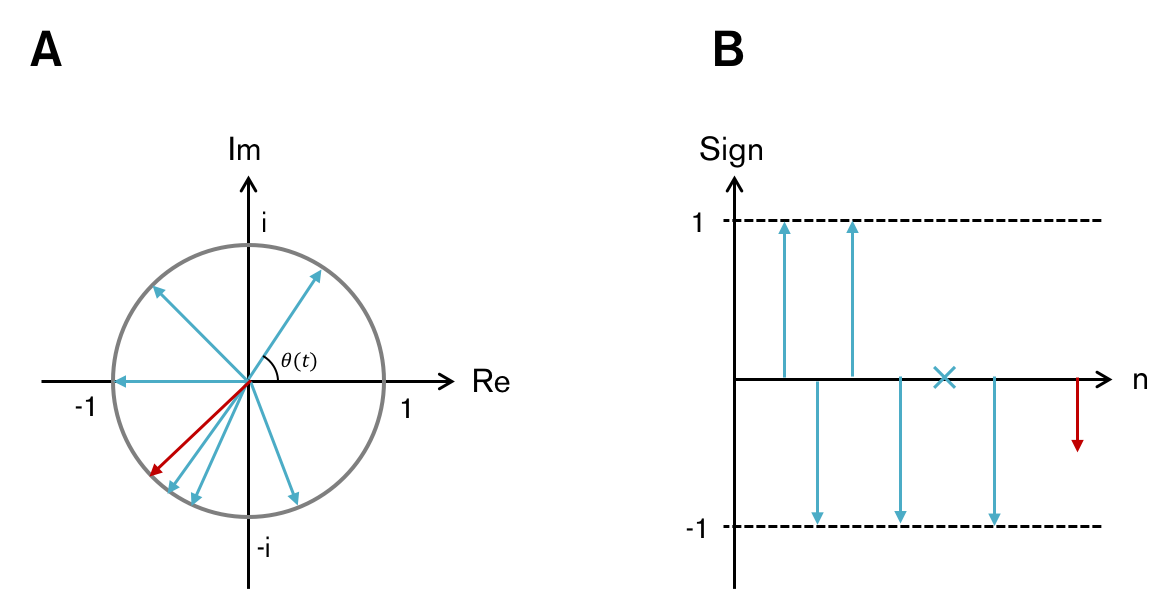
\includegraphics[width=\linewidth]{./images/chapter3/phase.png}\caption{Graphical descrptions of the phase coupling methods. Panel A shows the Phase Locking Value (PLV; \citealp{Lachaux1999}). On the Argrand diagram, the phase lags from a region of interest are represented by the blue arrows. The red arrow represents the PLV result. Note that the point which represents leakage at -π contributes to the final result. Panel B represents the Phase Lag Index (PLI; \citealp{Stam2007}). The same 6 phase lags have now been converted with the sign function, with the lag representing leakage now nullified (represented as the blue $\times$ at 0) so no longer contributes.}\label{fig_phase}
	\end{center}
\end{figure}

\section{Characterising signal leakage}\label{sec_signal_leakage}
\subsection{Analytic model}
In order to better understand the leakage effect, a simple analysis proves helpful. Consider the case of two sources: $\mathbf{q}_1$, which is of dimension $1 \times P$ and represents the timecourse at location $\mathbf{r}_1$. $\mathbf{q}_2$ shares the same dimensions and represents the timecourse at location $\mathbf{r}_2$. $P$ denotes the number of temporal samples in the data. $\mathbf{q}_1$ and $\mathbf{q}_2$ are assumed to be orthogonal, such that the covariance $\tfrac{1}{P}\mathbf{q}_1\mathbf{q}_2^T = 0$. Recalling the generative model in Section \ref{sec_gen_model}, if there are no other sources in the brain, then the $N \times P$ MEG data matrix can be described as:

\begin{equation}
\mathbf{m} = \mathbf{l}_1\mathbf{q}_1+\mathbf{l}_2\mathbf{q}_2 + \mathbf{e}, \label{eqn_leak_model_1}
\end{equation} where $\mathbf{l}_1$ and $\mathbf{l}_2$ (both of dimension $N \times 1$) are the forward solutions for sources $\mathbf{q}_1$ and $\mathbf{q}_2$ respectively. $\mathbf{e}$ shares the same dimensions as $\mathbf{m}$ and represents sensor noise. Using a source localisation technique (such as beamforming) to reconstruct $\mathbf{q}_1$:

\begin{equation}
\hat{\mathbf{q}}_1 = \mathbf{w}_1^T\mathbf{m} \label{eqn_leak_model_2}
\end{equation} where $\mathbf{w}_1$ represents the weights vector for location $\mathbf{r}_1$. Substituting Equation \ref{eqn_leak_model_2} into \ref{eqn_leak_model_1} and using the linear constraint for beamformer weights that $\mathbf{w}^T\mathbf{l} = 1$ the reconstructed source $\hat{\mathbf{q}}_1$ can be represented as

\begin{equation}
	\begin{aligned}
	\hat{\mathbf{q}}_1 &= \mathbf{w}_1\mathbf{l}_1\mathbf{q}_1 + \mathbf{w}_1^T\mathbf{l}_2\mathbf{q}_2 \\
	&= \mathbf{q}_1 + \mathbf{w}_1^T\mathbf{l}_2\mathbf{q}_2.
	\end{aligned}\label{eqn_leak_model_3}
\end{equation} What this means is that the beamformer reconstruction for source 1 is only independent of source 2 if $\mathbf{w}^T_1\,\mathbf{l}_2=0$. Similarly, reconstructing source 2 gives

\begin{equation}
\hat{\mathbf{q}}_2 = \mathbf{q}_2 + \mathbf{w}_2^T\mathbf{l}_1\mathbf{q}_1.\label{eqn_leak_model_4}
\end{equation} Given that the two sources are independent, it follows that the source leakage, $s$, can be generated by calculation of the covariance between the two reconstructed timecourses (i.e $s=\tfrac{1}{P}\hat{\mathbf{q}}_1\hat{\mathbf{q}}_2^T$). Substitution of Equations \ref{eqn_leak_model_3} and \ref{eqn_leak_model_4} gives

\begin{equation}
\begin{aligned}
s &= \tfrac{1}{P}\hat{\mathbf{q}}_1\hat{\mathbf{q}}_2^T \\
&= \tfrac{1}{P}\Big(\mathbf{q}_1 + \mathbf{w}_1^T\mathbf{l}_2\mathbf{q}_2\Big)\Big(\mathbf{q}_2 + \mathbf{w}_2^T\mathbf{l}_1\mathbf{q}_1\Big)^T\\
&= \tfrac{1}{P}\Big(\underbrace{\mathbf{q}_1\mathbf{q}_2^T}_\text{=0}+\mathbf{q}_1\mathbf{w}_2\mathbf{l}_1^T\mathbf{q}_1^T+\mathbf{q}_2^T\mathbf{w}_1^T\mathbf{l}_2\mathbf{q}_2+\underbrace{\mathbf{w}_1^T\mathbf{l}_2\mathbf{q}_2\mathbf{w}_2\mathbf{l}_1^T\mathbf{q}_1^T}_{=0}\Big) \\
&=\mathbf{w}_2^T\mathbf{l}_1\nu_1+\mathbf{w}_1^T\mathbf{l}_2\nu_2,
\end{aligned}\label{eqn_leak_model_5}
\end{equation} where $\nu_1=\tfrac{1}{P}\mathbf{q}_1\mathbf{q}_1^T$ and $\nu_2=\tfrac{1}{P}\mathbf{q}_2\mathbf{q}_2^T$. What this model shows is that the leakage term will only drop to zero if the weights of one source are orthogonal to the forward solution to the other source and vice versa. It should be noted that this model assumes zero noise (i.e the noise term from Equation \ref{eqn_leak_model_1} has been ignored), however in practice the addition of sensor noise will lower the covariance between sources (and therefore the leakage) so Equation \ref{eqn_leak_model_5} represents and upper limit on leakage between two sources.

\subsection{Simulations}
It proves instructive to extend this model in simulation. The simulations were based on a two source model equivalent to that described above. In all cases a seed source ($\mathbf{q}_2$) was placed approximately in the right primary sensorimotor cortex. 2781 iterations of the simulation were run, and on each iteration the test source ($\mathbf{q}_1$) was simulated in a different voxel. Voxels were placed on an 8 mm cubic grid spanning the entirety of brain space. Dipole orientation was allowed to vary smoothly with position in order to mimic dipole orientations in real MEG data. The source magnitudes were 8 nAm and source timecourses were generated from a beamformer reconstruction of a resting state MEG experiment. Source timecourses were phase randomised (\citealp{Prichard1994}; see Section \ref{phase_randomisation} for a mathematical description) so as to have zero (or as little as possible) correlation between them. The geometry for the simulation were based on the CTF MEG system in Nottingham operating in third order synthetic gradiometer configuration. The location of the MEG sensors with respect to brain anatomy was based on a real experimental recording session. Two separate noise models were used, in case 1, sensor noise was drawn from a Gaussian random process (meaning noise was uncorrelated across sensors). In case 2, real MEG noise was employed (where interference is correlated across MEG sensors). This was generated via the recording of 300 s of real MEG data with no subject in the system. 

The results of this simulation are shown in Figure \ref{figure_3_1}. Figure \ref{figure_3_1}A shows images of the magnitude of leakage between the seed source, and test sources at all other locations in the brain. The top two rows shows shows Gaussian sensor noise whereas the bottom rows shows realistic noise. The group of 4 images shows the analytical case (which reflects an upper limit on leakage based on Equation \ref{eqn_leak_model_5}) the results from the actual simulation. Note that in all cases source leakage is at its worst in brain areas adjacent to the seed. Note also that leakage worsens when using a realistic noise model. Figure \ref{figure_3_1}B shows equivalent leakage images for shallow (left) and deep (right) grey matter sources. It is clear that source leakage worsens for deeper sources due to their lower signal to noise ratio. Finally in Figure \ref{figure_3_1}C the upper panel shows the relationship between the analytical model in Equation \ref{eqn_leak_model_5}, and the actual simulation where the analytical model gives an upper limit on leakage. The lower panel of Figure \ref{figure_3_1}C shows leakage magnitude as a function of Euclidian distance between the seed and test voxels. Note that even sources separated by as much as 5 cm can exhibit a large amount of signal leakage, which would significantly confound any attempt at functional connectivity analysis. As shown by the above simulation, signal leakage differs depending on the brain area being studied, the signal to noise ratio of the data and the sensor level noise model. In addition, it depends on the inverse solution being used \citep{Scoffelen2009}, and the number of dipoles active in the brain. As can be seen from the images in Figure \ref{figure_3_1}A, the spatial profile of leakage is asymmetric around the seed location.

\begin{figure}[h!]
	\begin{center}
		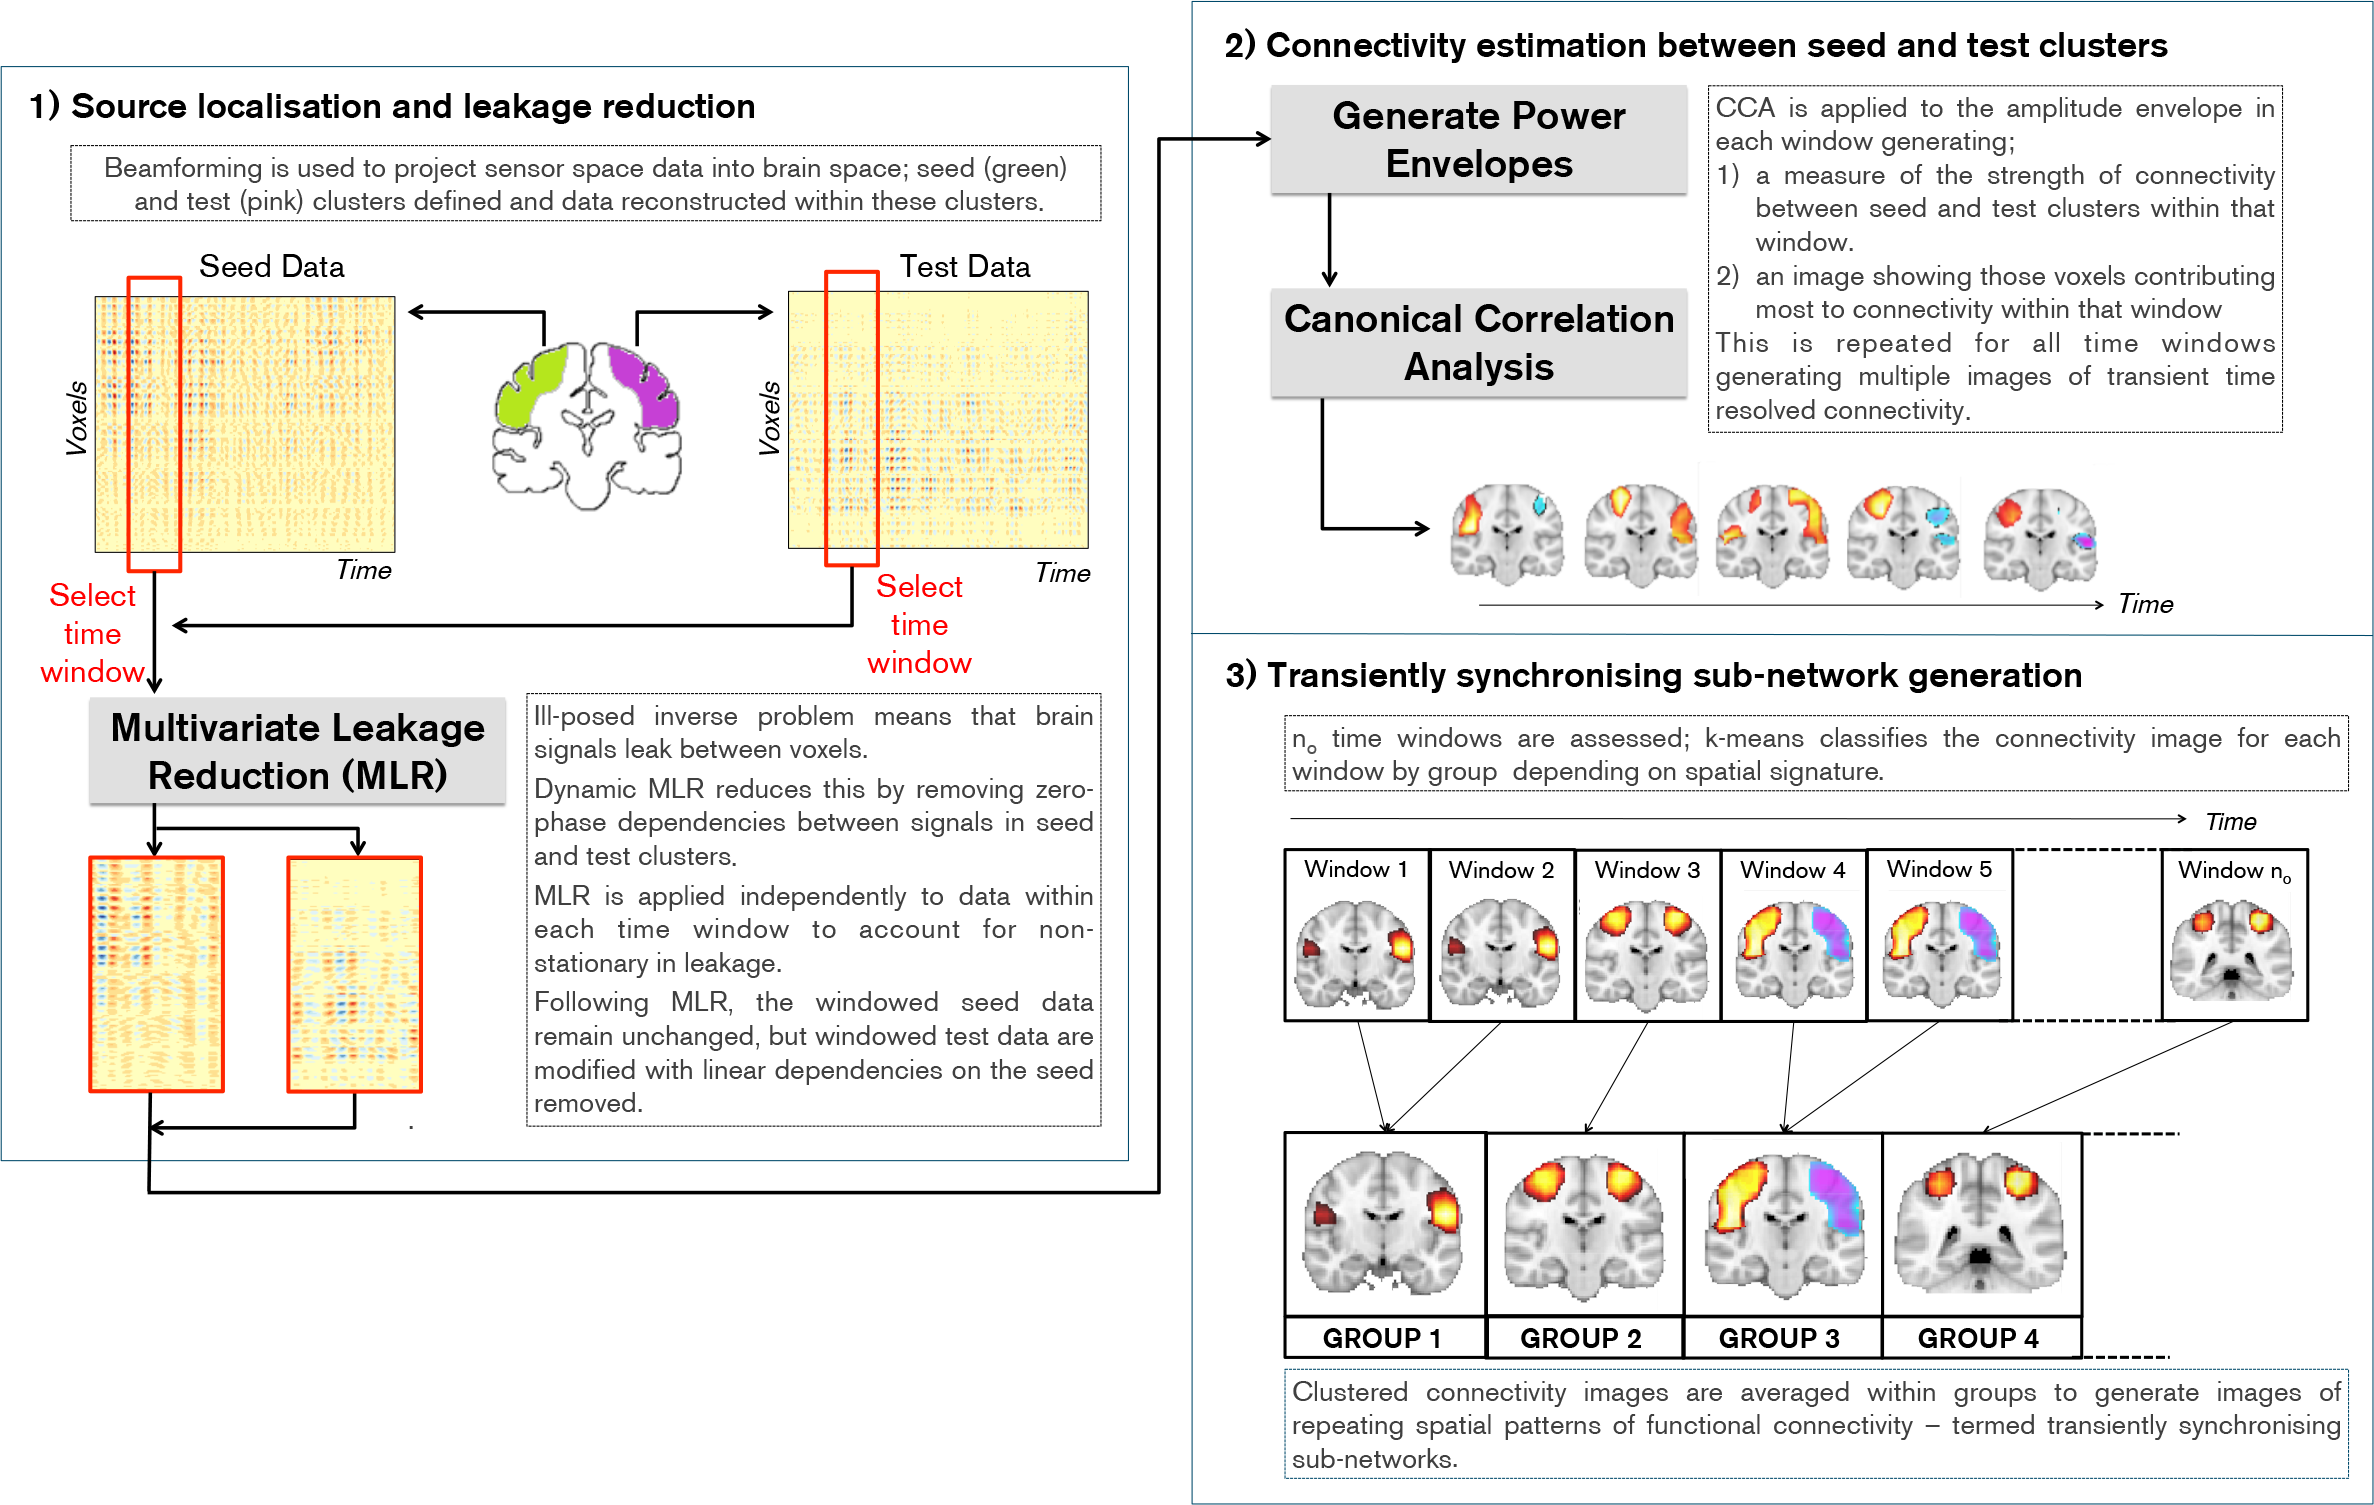
\includegraphics[width=\linewidth]{./images/chapter3/Figure_1.png}\caption{Examples of source space signal leakage. A) Images showing the magnitude of leakage between a simulated source in the primary sensorimotor cortex (blue dot), and equivalent simulated sources placed at all other brain locations. The upper panels show the analytical worst-case scenario whereas the lower panels show results from the actual simulation. The upper panels shows simulated Gaussian sensor level noise (i.e. the noise is uncorrelated across channels) whereas the lower panels shows realistic noise (which is correlated across the channels). Note in all cases that source leakage is worst close to the seed and typically spreads asymmetrically around the seed. Note also that leakage worsens with a realistic noise model. B) Equivalent images for a shallow cortical source (left) and a deep source (right); leakage worsens for deeper sources which exhibit a lower signal to noise ratio. C) Upper panel shows the relation between the analytical model in Equation 9, and the actual simulation for every test voxel; note the analytical model gives a “worst case scenario” regarding the leakage, which is reduced in the simulation via the addition of sensor level noise. The lower panel shows leakage magnitude as a function of Euclidian distance between the seed and the test voxels.\label{figure_3_1}}
	\end{center}
\end{figure}
\clearpage

\section{Correcting for signal leakage}\label{sec_signal_corr}
A number of potential solutions to the source leakage problem have been proposed \citep{Nolte2004,Stam2007,Brookes2012b,Hipp2012,Ewald2012,Marzetti2013,Brookes2014,ONeill2015A,Colclough2015,Wens2015} Although separate methods have different modes of operation, they are all based on the observation that leakage generates altered connectivity between estimated sources, which manifests as a zero-phase-lag correlation. Indeed this is shown by Equations \ref{eqn_leak_model_3} and \ref{eqn_leak_model_4}, which imply that leakage results in a weighted addition of a distal source. Genuine connectivity, on the other hand, is more likely to incorporate a time lag, generated as electrical signals travel between different brain regions. This means that elimination of all zero-phase-lag correlations in source space should result in the elimination of leakage, albeit at the expense of a loss of genuine zero-phase-lag connectivity (which has been shown to exist in invasive recordings; \citealp{Singer1999}). The application of beamforming supresses temporally correlated sources and this potentially aids leakage reduction. However for such suppression to occur, sources must be highly correlated ($r > \sim 0.7$ – which is unlikely for anything other than driven steady state responses) and therefore even after beamforming, further steps must be taken if leakage artefacts are to be controlled. In phase based connectivity metrics, leakage reduction methods usually circumvent zero-phase (and conversely π-phase) connections by assessing only the imaginary part of a signal in the Fourier domain \citep{Nolte2004,Nolte2008,Ewald2012,Marzetti2013} or by focusing on the asymmetry of the phase difference distribution \citep{Stam2007,Vinck2011}. In the case of metrics which employ amplitude data, methods have been derived to regress out the zero-phase relationship at source level, prior to connectivity analysis.

\subsection{Pairwise regression}
Consider again two beamformer estimated timecourses $\hat{\mathbf{q}}_1$ and $\hat{\mathbf{q}}_2$ representative of two underlying sources with a linear zero-phase-lag relationship caused by leakage. To mitigate the leakage, a linear projection of the seed voxel, $\hat{\mathbf{q}}_2$, is removed from the test voxel $\hat{\mathbf{q}}_1$. Mathematically, a general linear model is applied such that

\begin{equation}
\hat{\mathbf{q}}_1 = \beta\hat{\mathbf{q}}_2 + \hat{\mathbf{q}}_{1M}
\end{equation} where $\beta$ represents the effect size and relates directly to the magnitude of the leakage. $\hat{\mathbf{q}}_{1M}$ is the residual measurement, which represents the leakage-suppressed timecourse for the test location (i.e $\hat{\mathbf{q}}_{1M}$ is the beamformer estimate of activity in $\hat{\mathbf{q}}_1$, but with the linear dependence on $\hat{\mathbf{q}}_{2}$ [leakage] removed). $\beta$ can be estimated as.

\begin{equation}
\beta = \hat{\mathbf{q}}_1\hat{\mathbf{q}}_2^+ \label{eqn_3_7}
\end{equation} where the superscript $+$ denotes the Moore-Penrose pseudo-inverse. 

Figure \ref{figure_3_2} shows an example of envelope based functional connectivity taken from a real MEG recording in a single subject. Five minutes of MEG data were recorded using the CTF MEG system in Nottingham (note: these data were first presented in a study by \cite{Brookes2011a}). The subject was asked to lie in the system and “think of nothing” whilst connectivity was assessed, over all time, between a seed location in left sensorimotor cortex and all other voxel locations in the brain. In the upper panel, connectivity was computed between the seed and all other test voxels with no leakage reduction applied. In the lower panel, leakage reduction has been employed using the method outlined above. In both cases, envelopes of beta band (13-30 Hz) oscillations were employed. It is clear that a functional network of brain regions exists in the data, with the beta band envelope in left motor cortex showing high levels of correlation with equivalent envelopes in homologous regions of right sensorimotor cortex. In addition, note the significant advantages afforded by the reduction in zero-phase-lag correlation. In the uncorrected case, regions showing high connectivity extend from the seed voxel towards the centre of the brain as well as into the left temporal lobe. The spatial profile of leakage is in good agreement with the simulation presented in Figure \ref{figure_3_1}. This blurring around the seed location is reduced when applying leakage reduction.  

\clearpage

\begin{figure}[h!]
	\begin{center}
		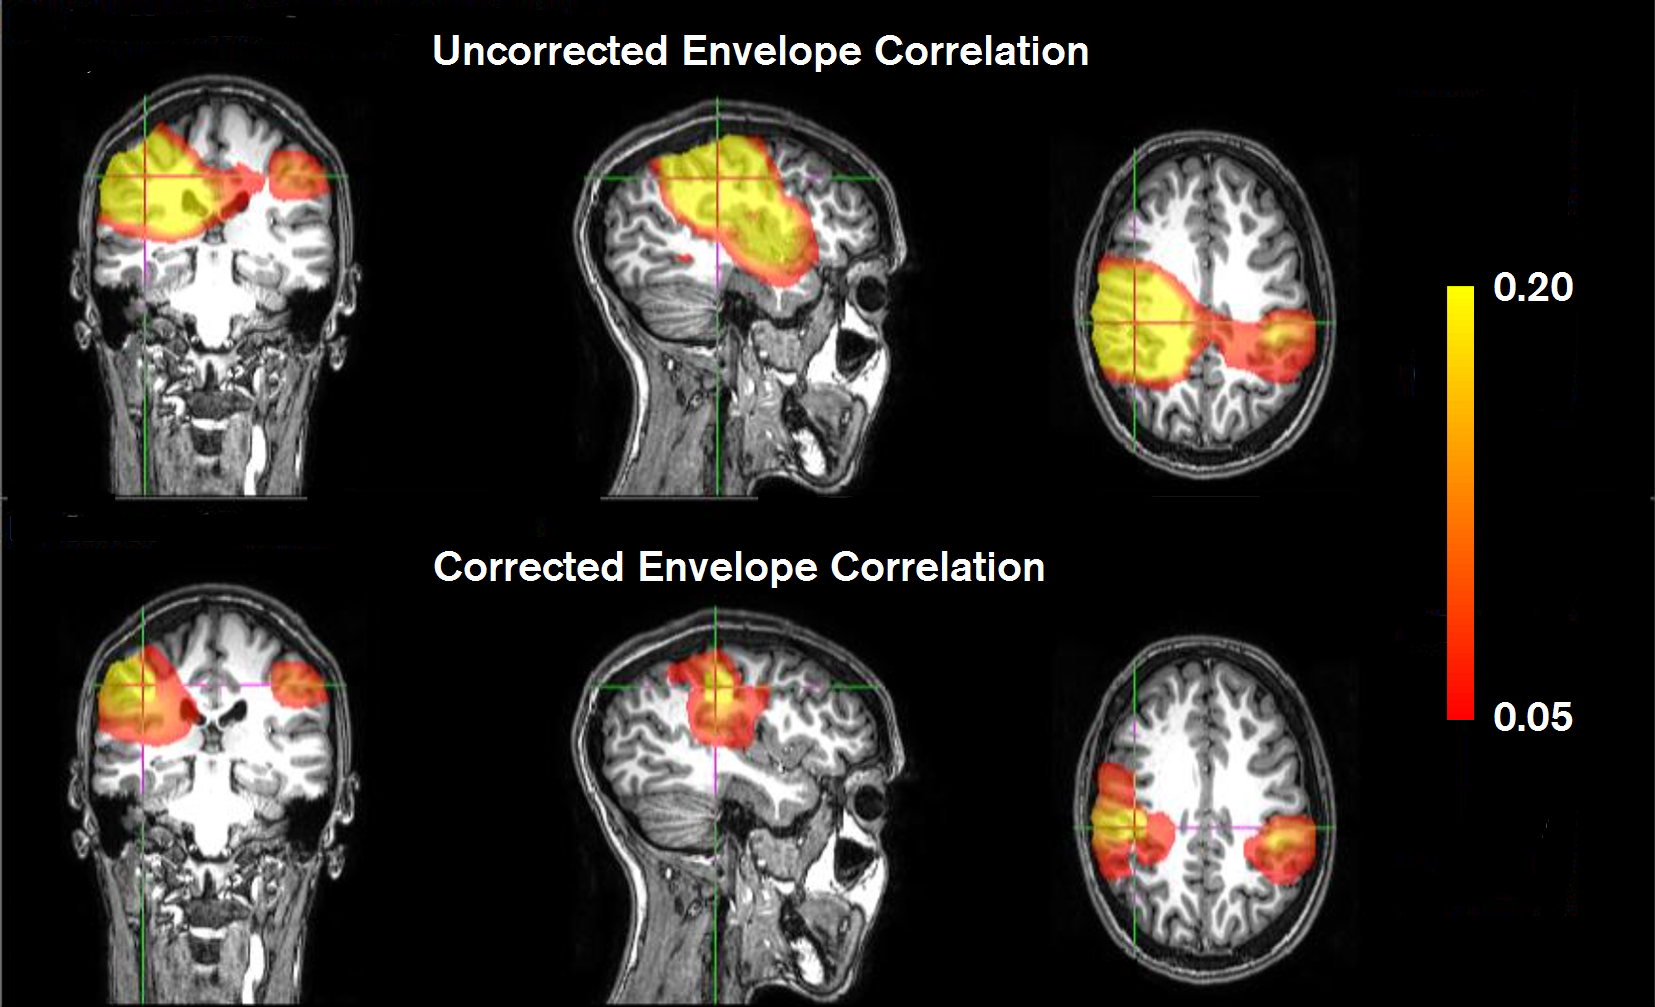
\includegraphics[width=\linewidth]{./images/chapter3/Figure_2.png}\caption{An illustration of leakage correction. Top Panel: Envelope correlation in real data between a seed in right motor cortex and all other brain locations, prior to reduction of leakage. Bottom Panel: Envelope correlation for the same data, post leakage reduction.\label{figure_3_2}}
	\end{center}
\end{figure}


\subsection{Limitations and signal kurtosis}

Despite the advantages of leakage reduction strategies, they have significant limitations, which should be discussed. Firstly, the pairwise method does not make the modified test timecourse, $\hat{\mathbf{q}}_{1M}$, a faithful reconstruction of the true source timecourse $\hat{\mathbf{q}}_1$. In fact, the modified timecourse retains an element of leakage from $\hat{\mathbf{q}}_2$. Only the magnitude of that leakage is altered, in such a way as to ensure orthogonality between $\hat{\mathbf{q}}_{1M}$ and $\hat{\mathbf{q}}_2$. To demonstrate this recall Equations \ref{eqn_leak_model_3} and \ref{eqn_leak_model_4}, the reconstructed sources $\hat{\mathbf{q}}_1$ and $\hat{\mathbf{q}}_2$ are defined as

\begin{equation}
\begin{aligned}
\hat{\mathbf{q}}_1 &=\mathbf{q}_1 +a\mathbf{q}_2 \\
\hat{\mathbf{q}}_2 &=\mathbf{q}_2 +b\mathbf{q}_1
\end{aligned}
\end{equation} where $a = \mathbf{w}^T_1\mathbf{l}_2$ represents the leakage from the seed source $\mathbf{q}_2$ to the test $\mathbf{q}_1$ and $b = \mathbf{w}^T_2\mathbf{l}_1$ is the leakage in the opposite direction. Using the leakage reduction algorithm described above the leakage estimate, $\beta$ is given by a Moore Penrose pseudoinverse, thus:

\begin{equation}
\begin{aligned}
\beta &= \big[\hat{\mathbf{q}}_2^T\hat{\mathbf{q}}_2\big]^{-1}\hat{\mathbf{q}}_2^T\hat{\mathbf{q}}_1\\
&=\big[(\mathbf{q}_2+b\mathbf{q}_1)^T(\mathbf{q}_2+b\mathbf{q}_1)\big]^{-1}(\mathbf{q}_2+b\mathbf{q}_1)^T(\mathbf{q}_1+a\mathbf{q}_2).
\end{aligned}
\end{equation} If $\mathbf{q}_1$ and $\mathbf{q}_2$ are temporally uncorrelated such that $\mathbf{q}_1^T\mathbf{q}_2 = \mathbf{q}_2^T\mathbf{q}_1 = 0$ , then:

\begin{equation}
\begin{aligned}
\beta &= \big[\mathbf{q}_2^T\mathbf{q}_2+b^2\mathbf{q}_1^T\mathbf{q}_1\big]^{-1}(a\mathbf{q}_2^T\mathbf{q}_2+b\mathbf{q}_1^T\mathbf{q}_1)\\
&=\frac{a\sigma_2+b\sigma_1}{\sigma_2+b^2\sigma_1}
\end{aligned}
\end{equation} where $\mathbf{q}_1^T\mathbf{q}_1 = \sigma_1$ and likewise $\mathbf{q}_2^T\mathbf{q}_2 = \sigma_2$. Having found $\beta$, it becomes possible to derive an equation for the modified estimated source timecourse ($\hat{\mathbf{q}}_{1M}$) following leakage reduction:

\begin{equation}
\begin{aligned}
\hat{\mathbf{q}}_{1M} &= \hat{\mathbf{q}}_{1} - \beta\hat{\mathbf{q}}_{2}\\
&= (\mathbf{q}_{1} + a\mathbf{q}_{2})-\Bigg[\frac{a\sigma_2+b\sigma_1}{\sigma_2+b^2\sigma_1}\Bigg](\mathbf{q}_{2} + b\mathbf{q}_{1}).
\end{aligned}
\label{eqn_dyn_leak_0}
\end{equation}Which simplifies to

\begin{equation}
\hat{\mathbf{q}}_{1M} = k(\sigma_2\mathbf{q}_1 - b\sigma_1\mathbf{q}_2),
\end{equation} where $k = \frac{1-ab}{\sigma_2+b^2\sigma_1}$ is a constant. This shows that leakage reduction applied in this way does not mean that $\hat{\mathbf{q}}_{1M}$ is a corrected and hence faithful reconstruction of $\mathbf{q}_1$. Rather, it ensures $\hat{\mathbf{q}}_{1M}$ and $\hat{\mathbf{q}}_{2}$ are orthogonal. Second, as noted earlier, the method also means the removal of true zero-phase connections; this is important, particularly given that invasive recordings show significant genuine zero-phase-lag effects in the brain (Singer, 1999). 

Finally, for the regression method to work, the data need to be Gaussian distributed. This is highlighted in Figure 5B which shows results from a simple simulation. Two signals, $\mathbf{X}$ and $\mathbf{Y}$, were generated as linear mixtures of independent timecourses, $\mathbf{S}_1$ and $\mathbf{S}_2$. The first mixture was defined as $\mathbf{X}=\mathbf{S}_1-k\mathbf{S}_2$ and the second as $\mathbf{Y}=\mathbf{S}_2+k\mathbf{S}_1$. The parameter $k$ is a positive constant and controls the degree of leakage in the simulation; this was set to 0.2. Three separate simulations were undertaken in which $\mathbf{S}_1$ and $\mathbf{S}_2$ were drawn from a) Gaussian distributed noise b) leptokurtic noise (Gaussian\textsuperscript{3}) and c) uniformly distributed platykurtic noise. Leakage reduction was applied to \textbf{Y} and the result should be zero correlation between timecourses following correction. A phase randomisation approach \citep{Prichard1994} was employed to test the significance of any non-zero correlation observed and the false positive count was calculated as the number of significant measures of correlation observed across 1000 iterations of the simulation. Results show clearly that if the underlying processes ($\mathbf{S}_1$ and $\mathbf{S}_2$) are normally distributed, the false positive rate (FPR) follows the expected trend (black line). However, if $\mathbf{S}_1$ and $\mathbf{S}_2$ are either leptokurtic or platykurtic, leakage is poorly accounted for. Overall, the Gaussian assumption is reasonable; indeed it is an assumption at the heart of many of the source localisation methodologies employed in MEG. However situations exist where this is not the case, for example epileptic seizures \citep{Prendergast2013} and for this reason care should be taken when deploying the regression method to correct for leakage.

However it should be noted that considering the extensive coverage of orthogonalisations shortcomings, it is a powerful tool which vastly improves our estimates of functional connectivity analysis, and should be utilised in all MEG connectivity analyses.  

\begin{figure}[h!]
	\begin{center}
		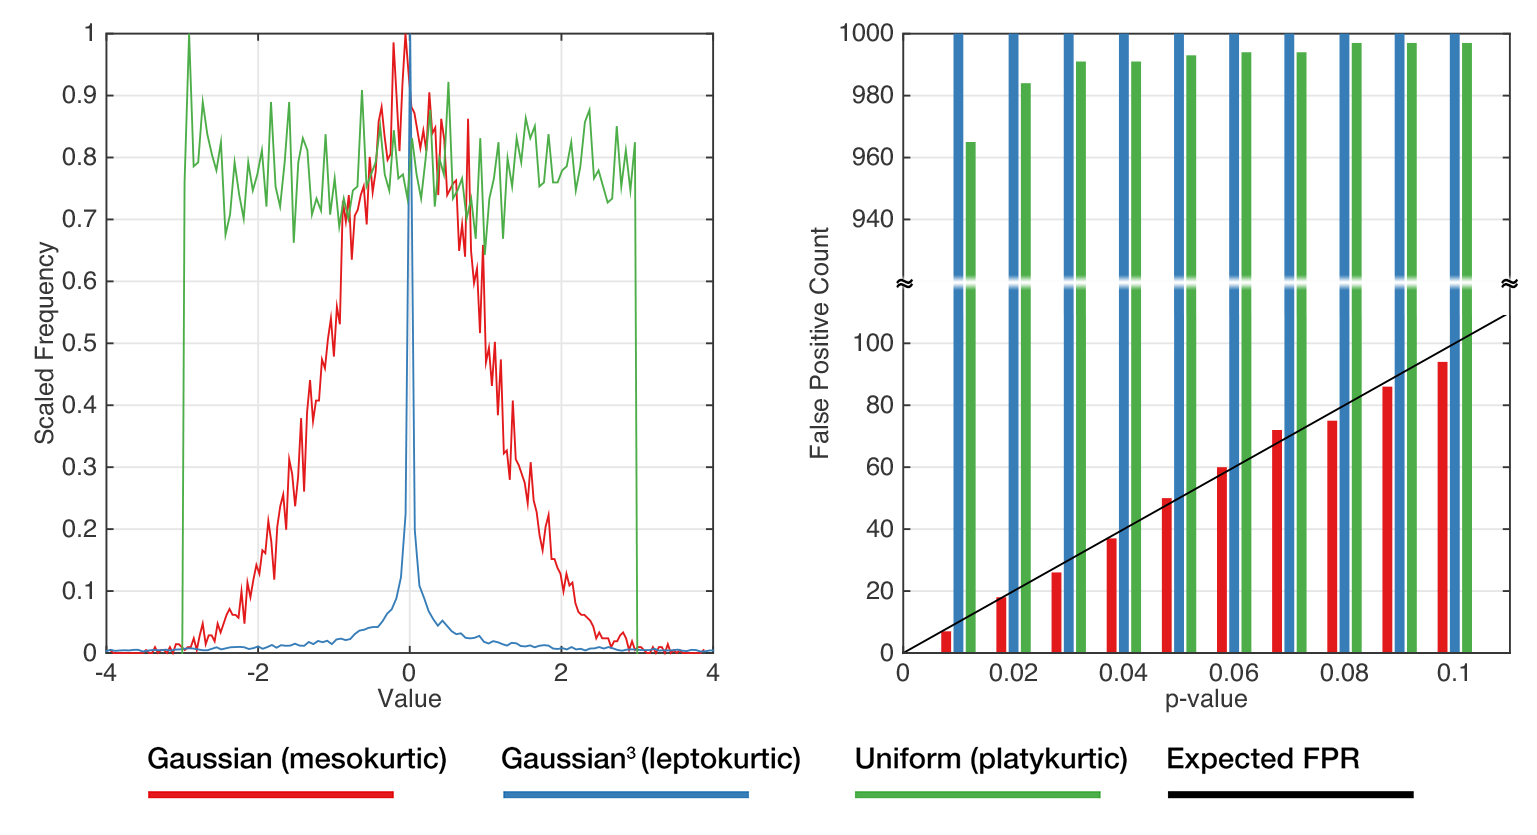
\includegraphics[width=\linewidth]{./images/chapter3/kurtosis.png}\caption{Results of a simulation characterising the effectiveness of linear
			regression as a technique for leakage reduction. Left: The statistical distributions used
			to generate the underlying independent timecourses \textbf{S}1 and \textbf{S}2. Right: The false positives
			detected and compared to the theoretical values. Note that only underlying Gaussian
			distributed data result in agreement between the calculated and theoretical false positive
			rates and the other distributions return false positives over 96\% of the time. \label{figure_3_kurt}}
	\end{center}
\end{figure}

\clearpage
\subsection{Symmetric orthogonalisation}\label{sec_symm_orth}
In a connectivity analysis where we want to compare \textit{n} timecourses to each other to assess $n^2$ connections simultaneously (such as in Chapter \ref{chap_atlas}), pairwise orthogonalisation is not the ideal candidate to correct across all pairs simultaneously. It could be suggested that we could orthogonalise sequentially between pairs, however it poses the question of how to best approach this. In a simple case where orthogonalisation is performed between an ROI and a random (currently uncorrected) ROI, then there are (in this case) \textit{n}! possible combinations, which at $n=58$ becomes a number which is approximately the total atoms in the observable universe. Also it is not a symmetric correction to the data; that is to say the correction of source 1 based on source 2 is not equal to correcting in the opposite direction, this is shown in Figure \ref{figure_3_2a}B, where in a simple 2-dimensional case it can be clearly seen. This again could potentially prove to be a hindrance if we are assessing connections between multiple ROIs, as we have to ensure no ROI timecourses share a zero-phase relationship with any other. An elegant solution was  proposed recently by \cite{Colclough2015}, which attempts to symmetrically orthogonalise all timecourses. This method, based upon Lödwdin's symmetric orthogonalisation \citep{Lowdin1950,Mayer2002} is able to reduce linear relations between multiple separate timecourses in one calculation. The proof for this can be found in one of the aforementioned references but a description of the algorithm follows. Assume you have a measurement matrix \textbf{M}, comprising an $n \times s$ array where \textit{n} is the number of timecourses you wish to orthogonalise and \textit{s} is the number of temporal samples in each timecourse. A singular value decomposition of \textbf{M} yields

\begin{equation}
\mathbf{M}=\mathbf{USV}^T,
\end{equation} where the columns of \textbf{U} are the eigenvectors of $\mathbf{MM}^T$, the columns of \textbf{V} are the eigenvectors of $\mathbf{M}^T\mathbf{M}$ and the diagonal elements of \textbf{S} are the square root of the corresponding eigenvalues shared between \textbf{U} and \textbf{V}. To symmetrically orthogonalise all timecourses, we simply perform the calculation.

\begin{equation}
\mathbf{M}_O = \mathbf{UV}^T
\end{equation} The effect of symmetric orthogonalisation can be seen Figure \ref{figure_3_2a}C, where rather than one timecourse being adjusted like in Figure \ref{figure_3_2a}B, both are modified by the same amount. Although this might be considered a more ‘aggressive’ procedure (i.e. the resulting timecourses may be further from the original beamformed data than might be the case for pairwise correction), this technique
should be considered the method of choice for inter-regional all-to-all metrics of functional
connectivity. However it should be noted that for symmetric orthogonalisation to be correctly implemented, the number of timecourses being orthogonalised must be lower or equal to the rank of \textbf{M}; in the case of MEG data from Nottingham this corresponds to approximately the number of sensors which were used to beamform the data. This means it cannot be used in situations such as placing a seed in a voxel and investigating its connectivity to the rest of the brain volume, where the connections vastly outnumber the data rank. However in that situation as we are only interested in the influence of one voxel timecourse on the rest of the brain a pairwise correction is sufficient. 

\begin{figure}[h!]
	\begin{center}
		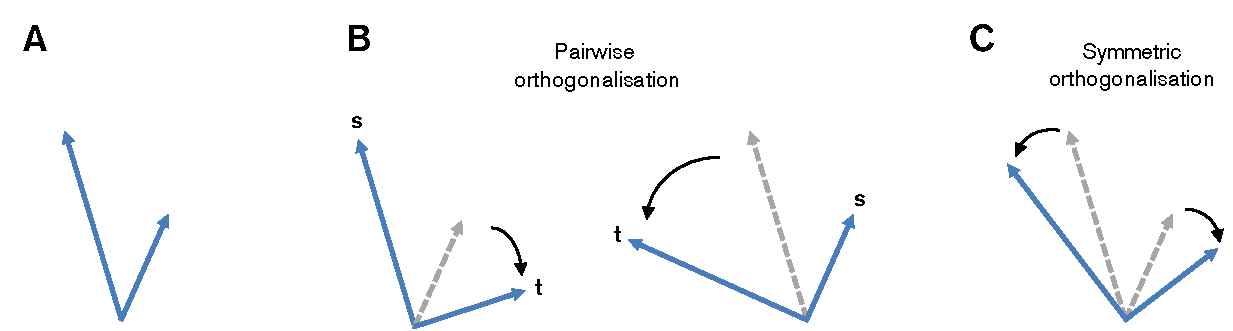
\includegraphics[width=\linewidth]{./images/chapter3/orthogonal.pdf}\caption{A diagram to show the effect of different leakage reduction algorithms on a two vector system. A) The two vectors showing a linear relationship. B) The effect of using the pairwise corrections methods \citep{Brookes2012b}, showing the two differing results depending on the selection of the seed \textbf{s} and test \textbf{t} vectors. C) The result of the symmetric orthogonalisation \citep{Colclough2015}, note that both vectors are modified by the same magnitude.\label{figure_3_2a}}
	\end{center}
\end{figure}

\section*{Summary}
In this chapter we have discussed the many technical facets of measuring functional connectivity in MEG. First, we introduced the measures of functional connectivity which allow us to quantify the strength of a relationship between two or more distal regions and showed that there are many approaches which a study can use before explaining that we shall use amplitude envelope coupling as our metric of choice for connectivity. Second we established that the ill posed nature of the MEG inverse problem can potentially confound results by artefactually inflating connectivity levels, and identified methods which can be used to reduce the effect this has. With all of this considered we can now proceed onto the experimental side of this thesis.
